%%%%%%%%%%%%%%%%%%%%%%%%%%%%%%%%%%%%%%%%%
% modul: 	intro
% topic:	recap
%%%%%%%%%%%%%%%%%%%%%%%%%%%%%%%%%%%%%%%%%

% ------------------------------------------------------------
%	PACKAGES AND THEMES
% ------------------------------------------------------------
\documentclass{beamer}

\mode<presentation> {

% The Beamer class comes with a number of default slide themes
% which change the colors and layouts of slides. Below this is a list
% of all the themes, uncomment each in turn to see what they look like.

%\usetheme{default}
%\usetheme{AnnArbor}
%\usetheme{Antibes}
%\usetheme{Bergen}
%\usetheme{Berkeley}
%\usetheme{Berlin}
%\usetheme{Boadilla}
%\usetheme{CambridgeUS}
%\usetheme{Copenhagen}
%\usetheme{Darmstadt}
%\usetheme{Dresden}
%\usetheme{Frankfurt}
%\usetheme{Goettingen}
%\usetheme{Hannover}
%\usetheme{Ilmenau}
%\usetheme{JuanLesPins}
%\usetheme{Luebeck}
\usetheme{Madrid}
%\usetheme{Malmoe}
%\usetheme{Marburg}
%\usetheme{Montpellier}
%\usetheme{PaloAlto}
%\usetheme{Pittsburgh}
%\usetheme{Rochester}
%\usetheme{Singapore}
%\usetheme{Szeged}
%\usetheme{Warsaw}

% As well as themes, the Beamer class has a number of color themes
% for any slide theme. Uncomment each of these in turn to see how it
% changes the colors of your current slide theme.

%\usecolortheme{albatross}
%\usecolortheme{beaver}
%\usecolortheme{beetle}
%\usecolortheme{crane}
%\usecolortheme{dolphin}
%\usecolortheme{dove}
%\usecolortheme{fly}
%\usecolortheme{lily}
%\usecolortheme{orchid}
%\usecolortheme{rose}
%\usecolortheme{seagull}
%\usecolortheme{seahorse}
%\usecolortheme{whale}
%\usecolortheme{wolverine}

%\setbeamertemplate{footline} % To remove the footer line in all slides uncomment this line
%\setbeamertemplate{footline}[page number] % To replace the footer line in all slides with a simple slide count uncomment this line

%\setbeamertemplate{navigation symbols}{} % To remove the navigation symbols from the bottom of all slides uncomment this line
}

\usepackage{graphicx} % Allows including images
\usepackage{booktabs} % Allows the use of \toprule, \midrule and \bottomrule in tables

\usepackage[utf8]{inputenc}

% ------------------------------------------------------------
%	TITLE PAGE
% ------------------------------------------------------------

\title[INTRO recap]{INTRO recap SW10} % The short title appears at the bottom of every slide, the full title is only on the title page

\author[Hoti, Wirtz]{
	Arbnor Hoti \textsuperscript{1} 
	\and Raphael Wirtz \inst{2}
}
\institute[hslu]{
	\textsuperscript{1} \textit{arbnor.hoti@stud.hslu.ch} \and
	\inst{2} \textit{raphael.wirtz@stud.hslu.ch}
	\\
	\medskip
	HSLU Hochschule Luzern
}

%\author{author}
%institute[] % Your institution as it will appear on the bottom of every slide, may be shorthand to save space
% {
% HSLU - Hochschule Luzern Technik \& Architektur \\ % Your institution for the title page
% \medskip
% \textit{} % Your email address
% }
\date{\today} % Date, can be changed to a custom date

\begin{document}

\begin{frame}
\titlepage % Print the title page as the first slide
\end{frame}

\begin{frame}
\frametitle{Inhaltsverzeichnis} % TOC slide
\tableofcontents %  \section{} and \subsection{} commands,  automatically printed on this slide
\end{frame}

% ------------------------------------------------------------
%	PRESENTATION SLIDES
% ------------------------------------------------------------

%------------------------------------------------
\section{Übersicht} % Section
%------------------------------------------------
\begin{frame}
	\frametitle{Übersicht}
	\begin{itemize}
		\item{Liniensensor, für Position auf der Linie}
		\item{Motor}
		\item{PID, um auf der Linie zu bleiben}
		\item{Quadratur Encoder, zur Bestimmung von Position und Geschwindigkeit}
	\end{itemize}
\end{frame}

%------------------------------------------------
\section{IR Sensor} % Section
%------------------------------------------------
\begin{frame}
	\frametitle{IR Sensor}
	\begin{itemize}
		\item{Sender: IR-LED}
		\item{Empfänger: Phototransistor}
		\item{Unterschiedliche IR Reflexion}
		\begin{itemize}
			\item{Unterscheidung zwischen Schwarz und Weiss}
		\end{itemize}
		\item{Energieversorgung über Akkumulatoren}
	\end{itemize}

	\begin{figure}[h!]
		\centering
		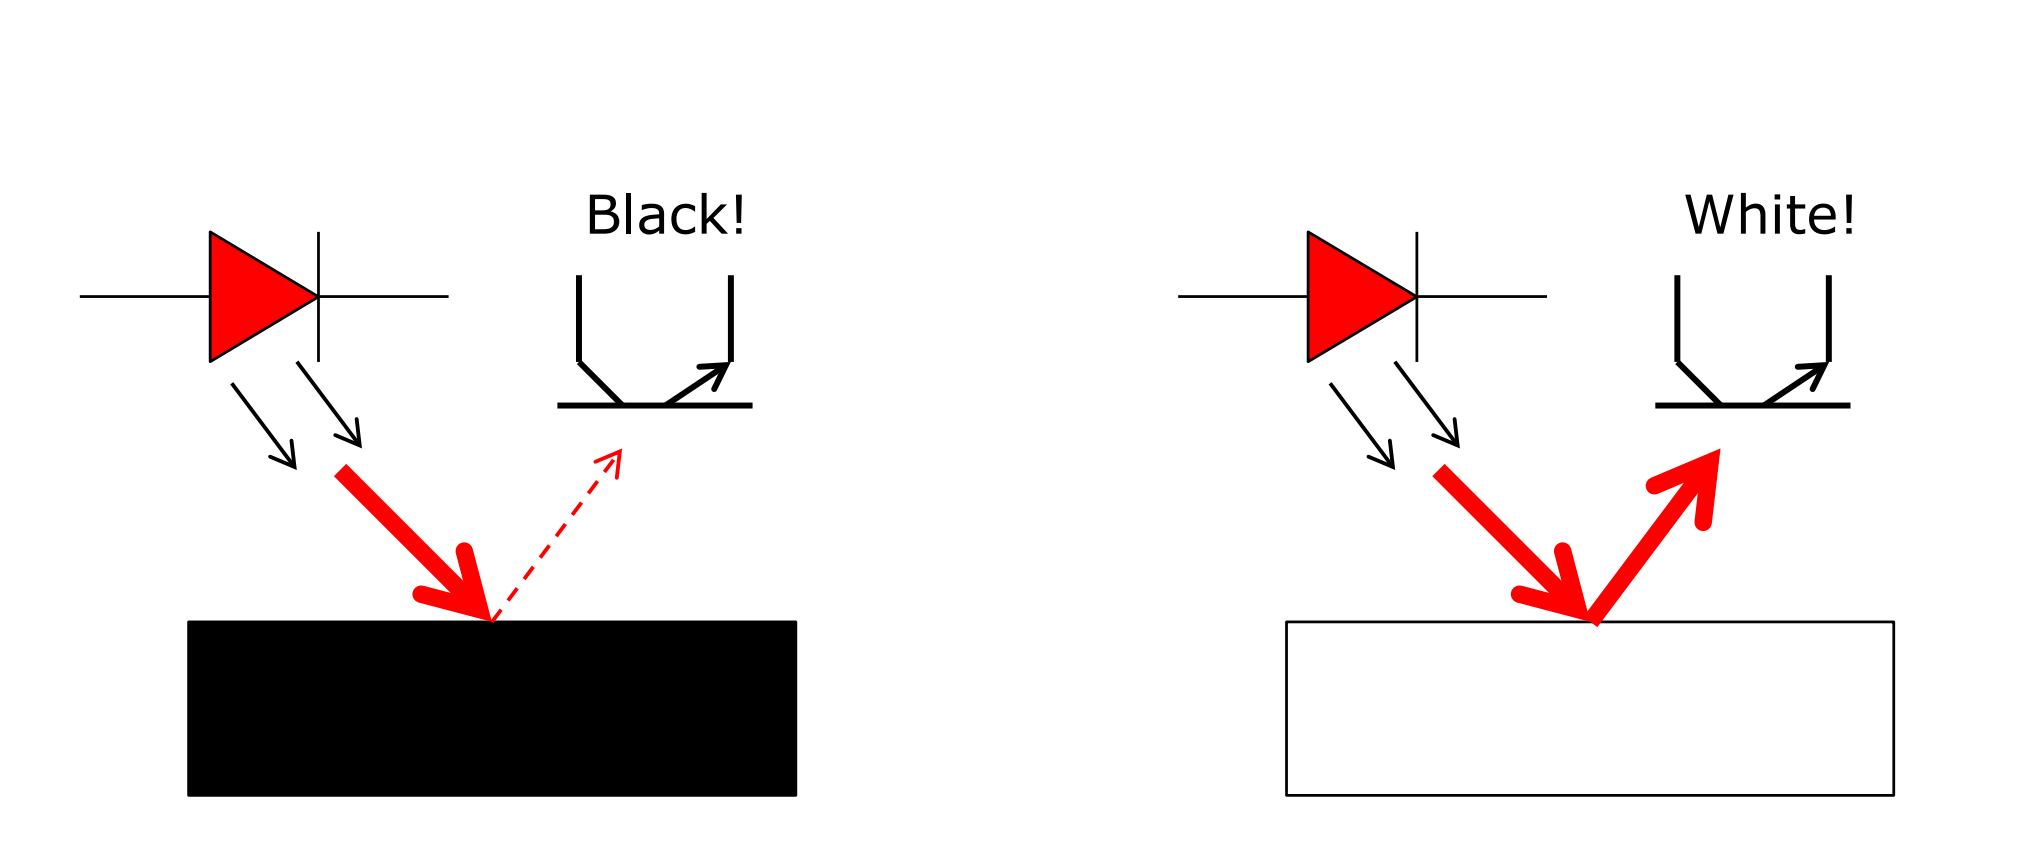
\includegraphics[width=0.6\linewidth]{figure/linefollowing_sensor_irLed_phototr.PNG}
	\end{figure}

	%\end{figure}
\end{frame}

\begin{frame}
	\frametitle{IR Sensor}
	\begin{itemize}
		%\item{Analoge Entladeschaltung !!!!Folie S11 abgleichen!!!!}
		\item{Transistoren werden über ein Array angesteuert}
		\begin{itemize}
			\item{Array ein-/ausschalten über Port $IR\_LED\_ON$ (via Jumper)}
		\end{itemize}
	\end{itemize}

	\begin{itemize}	
		\item{Störgrössen}
		\begin{itemize}
			\item{Crosstalk: IR LED sendet an falschen Transistor}
			\item{Externe Lichteinstreuung}
		\end{itemize}
	\end{itemize}

	\begin{figure}[h!]
		\centering
		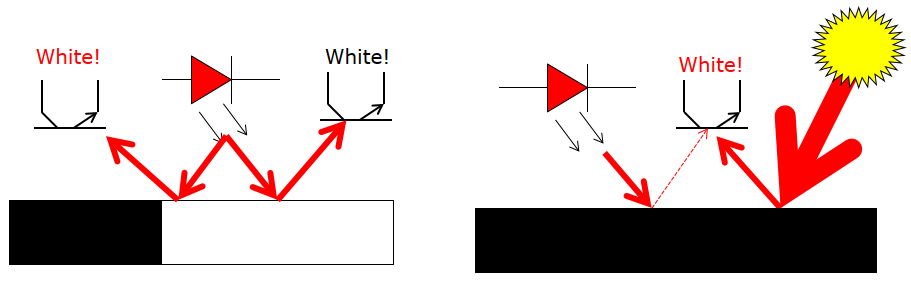
\includegraphics[width=0.6\linewidth]{figure/linefollowing_disturbance.PNG}
	\end{figure}
\end{frame}

% \begin{frame}
% 	\frametitle{Rohdaten und Kalibrierung}
% 	\begin{block}{Rohdaten}
% 		\begin{itemize}
% 			\item{Wert von Timer zwischen 0x0000 - 0xFFFF}
% 		\end{itemize}
% 	\end{block}

% 	\begin{block}{Kalibrierung}
% 		\begin{itemize}
% 			\item{Werte von Timer skalieren }
% 			\begin{itemize}
% 				\item{min Wert $\Rightarrow$ 0}
% 				\item{max Wert $\Rightarrow$ 1000}
% 			\end{itemize}
% 			\item{Neue Wertebereich zwischen 0 - 1000}
% 		\end{itemize}
% 	\end{block}
% \end{frame}

\begin{frame}
	\frametitle{Implementation}
	\begin{itemize}
		\item{Task, oder Prozess für Sensor}
		\item{Periodisches sampling, oder auf Abfrage\\
		$\Rightarrow$ Periodisches sampling für vorsehbares Systemverhalten (stabiles System)}
		\item{Kalibration}
		\begin{itemize}
			\item{min und max Werte skalieren zwischen 0 und 1000}
			\item{In Event, auf externen Befehl (Button, \dots)}
			\item{Daten im RAM gespeichert}
			\begin{itemize}
				\item{Nach jedem Neustart erneut Kalibration nötig \\
				$\Rightarrow$ Kalibrationdaten in Flash verschieben (nicht flüchtig)}
			\end{itemize}
		\end{itemize}
		%\item{State-machine (in Hauptapplikation)}

	\end{itemize}
	% Task or Process für Sensor
	% periodic sampling or on demand
	% Event für Kalibration
	% state-machine in main app
\end{frame}


%------------------------------------------------
\section{Motoren \& H-Brücke} % Section
%------------------------------------------------
\begin{frame}
	\frametitle{Motoren}
	\begin{itemize}
		\item{Geschwindikeit proportional zur Spannung (ohne Störgrössen)}
		\item{Störgrössen}
		\begin{itemize}
			\item{Mechanische Belastung}
			\item{Toleranzen im Antriebsstrang}
		\end{itemize}
	\end{itemize}

	\begin{exampleblock}{}
		\centering
		$\Rightarrow$ Regler
	\end{exampleblock}
	
\end{frame}

\begin{frame}
	\frametitle{H-Brücke}

	\begin{block}{Treiber IC (Dual H-Brücke) }
		\begin{itemize}
			\item{x = H-Bridge A,B\dots}
			\item{xENABLE: speed, via PWM}
			\item{xPHASE: direction, Vorwärts (1) und Rückwärts (0)}
			\item{MODE über Hardware auf 1 gesetzt}
		\end{itemize}
	\end{block}


	\begin{block}{Treiber Ansteuerung (motor.c)}
		 \begin{itemize}
	 		\item{xPHASE $\Leftarrow$ PWM}
	 		\item{xENABLE $\Leftarrow$ DIR}
	 		\item{Individuelles Ansteuern der Transistoren, exaktes Timing}
		 \end{itemize}
	\end{block}


	\begin{alertblock}{}
		Robo V1: Stützkondensatoren zu gering\\
		$\Rightarrow$ Spannungsversorgung sinkt bei Belastung.
	\end{alertblock}
	% others (emergency stop / Notbremse T2, T4 auf GND leitend NICHT IMPLEMENTIERT ? GRUND?)
	% für jeden Motor eine H-Brücke (über dual H-Bridge)
\end{frame}

\begin{frame}
		\frametitle{motor.c Interface}
		% \begin{block}{typedef enum}
		% 	MOT\_Direction : forward, backward\\
		% 	MOT\_MotorSide : left, right
		% 	% \begin{itemize}
		% 	% 	\item{MOT\_Direction : forward, backward}
		% 	% 	\item{MOT\_MotorSide : left, right }
		% 	% \end{itemize}
		% \end{block}
		
		\begin{block}{Funktionen}
			MOT\_SetDirection : DIR (boolean)\\
			MOT\_SetSpeedPercent : percent ($\pm$0-100) % +/- IST NICHT KORREKT (BUG FUER PRAESENTATION ;)
		%*MOT_GetMotorHandle(MOT_MotorSide side)
		\end{block}

		\begin{block}{}
			Gemeinsamer Wert für Geschwindikeit und Richtung\\ $\Rightarrow$ speed: (-100\% zu 100\%)
			\begin{itemize}
				\item{PWM: (0x0000-0xffff)}
				\item{DIR: (boolean)}
			\end{itemize}
		\end{block}

		\begin{alertblock}{}
			currSpeeedPercent: ist nicht die relative Geschwindigkeit gegenüber Unterboden!
		\end{alertblock}
\end{frame}
%------------------------------------------------
\section{Fragen} % Section
%------------------------------------------------
\begin{frame}
	\frametitle{Fragen}
	\begin{enumerate}
		\item{Weshalb kann der Motor nicht direkt mit einem PWM angesteuert werden?}
		\item{Welche Eingänge vom H-Brücken Treiber IC werden benötigt?}
		\item{Was ist der Vorteil, wenn die relative Geschwindikeit (\%)verwendet wird?}
		\item{Was muss aktiviert werden, damit die Phototransistoren verwendet werden können (Hardware)?}
		\item{Wieso wird eine Kalibierung gemacht?}
	\end{enumerate}
\end{frame}
%------------------------------------------------
\begin{frame}
	\frametitle{Fragen \& Antworten}
	\begin{enumerate}
		\item{Weshalb kann der Motor nicht direkt mit einem PWM angesteuert werden?}
		\\$\Rightarrow$ Ausgang liefert zu wenig Leistung.
		\item{Welche Eingänge vom H-Brücken Treiber IC werden von der Software angesteuert?}
		\\$\Rightarrow$ xENABLE, xPHASE
		\item{Was ist der Vorteil, wenn die relative Geschwindikeit (\%) verwendet wird?}
		\\$\Rightarrow$ Modularität, Relation zwischen Wirklichkeit und Software
		\item{Was muss aktiviert werden, damit die Phototransistoren verwendet werden können (Hardware)?}
		\\$\Rightarrow$ Sensor Array, Port $IR\_LED\_ON$ via Jumper setzen.
		\item{Wieso wird eine Kalibierung gemacht?}
		\\$\Rightarrow$ Normalisierte Werte
	\end{enumerate}
\end{frame}
%------------------------------------------------
\begin{frame}
	\begin{exampleblock}{Bug}
	\centering
		MOT\_SetSpeedPercent : percent (\textcolor{red}{$\pm$} 0-100)
	\end{exampleblock}
\end{frame}
%------------------------------------------------
\begin{frame}
	\Huge{\centerline{Outro}}
\end{frame}

\end{document}